% 4-12 题 图4_10：三边长R,√3R,2R的三角板在光滑圆环内平衡
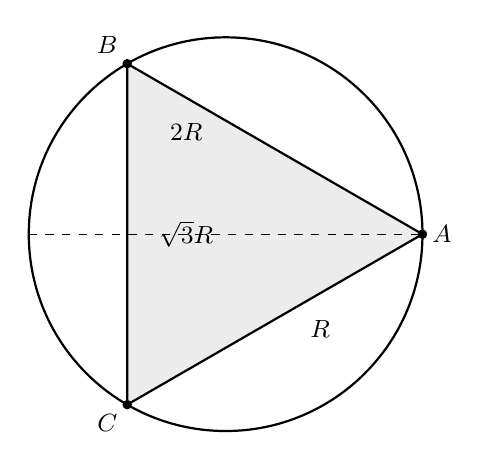
\begin{tikzpicture}[font=\small]
  % 圆环
  \draw[thick] (0,0) circle (2.5);
  % 三角板（30-60-90三角形，三边R,√3R,2R）
  % 取三角形顶点在圆周上
  % 边长比例 1 : √3 : 2，即30-60-90三角形
  % 将2R边（斜边）放在圆内某个位置
  \coordinate (A) at (2.5,0);              % 右侧顶点
  \coordinate (B) at ({-2.5*cos(60)},{2.5*sin(60)});  % 左上
  \coordinate (C) at ({-2.5*cos(60)},{-2.5*sin(60)}); % 左下
  \draw[thick, fill=gray!15] (A) -- (B) -- (C) -- cycle;
  % 顶点标注
  \filldraw (A) circle (1.5pt) node[right] {$A$};
  \filldraw (B) circle (1.5pt) node[above left] {$B$};
  \filldraw (C) circle (1.5pt) node[below left] {$C$};
  % 边长标注
  \node at (1.2,-1.2) {$R$};
  \node at (-0.5,0) {$\sqrt{3}R$};
  \node at (-0.5,1.3) {$2R$};
  % 水平直径（虚线）
  \draw[dashed] (-2.5,0) -- (2.5,0);
  % 角度θ（2R边与水平直径的夹角）
  \draw ({-2.5*cos(60)+0.15},{2.5*sin(60)+0.15}) node[above] {};
\end{tikzpicture}
